\subsection*{5.4 EXPERIMENT B: Localization Accuracy vs UWB Noise}
\noindent The second experiment evaluated the robustness of the I.C.U.M localization system with respect to increasing noise in UWB range measurements. While UWB generally provides high accuracy, real-world deployments are subject to non-line-of-sight conditions, multipath effects, and hardware limitations, all of which effectively increase measurement noise. The objective of this experiment was therefore to quantify the decay of the localization accuracy, as noise interfering with UWB readings increases.

\subsubsection*{Methodology}
\noindent To determine the accuracy limits of the proposed algorithm, we utilized a Centralized Global Solver. Unlike the real-time distributed approximation used in other experiments, this method performs a batch optimization on all collected range measurements. This provides a performance baseline for the algorithm on a fully connected graph, effectively benchmarking the best-case performance of the underlying physics model.

\noindent The experiment was conducted using the same simulation setup and system configuration as described in Section 5.3, ensuring validity across experiments. The focal metrics for this experiment were the $RMSE_{Aligned}$ and the standard deviation of the noise $\sigma$. A fixed node layout was deterministically set up across three different cases with a varying number of active nodes, while the noise level was increased repeatedly after every execution across a predefined range. For each noise level, the simulation was run for 600 seconds, after which the final localization metrics were recorded.

\noindent Figure \ref{fig:B_MAE} illustrates the relationship between UWB noise and final localization error for a fixed network size. Results are shown for small ($N = 3$), medium ($N = 8$), and larger ($N = 15$) node counts. 
\begin{figure}[h]
\centering
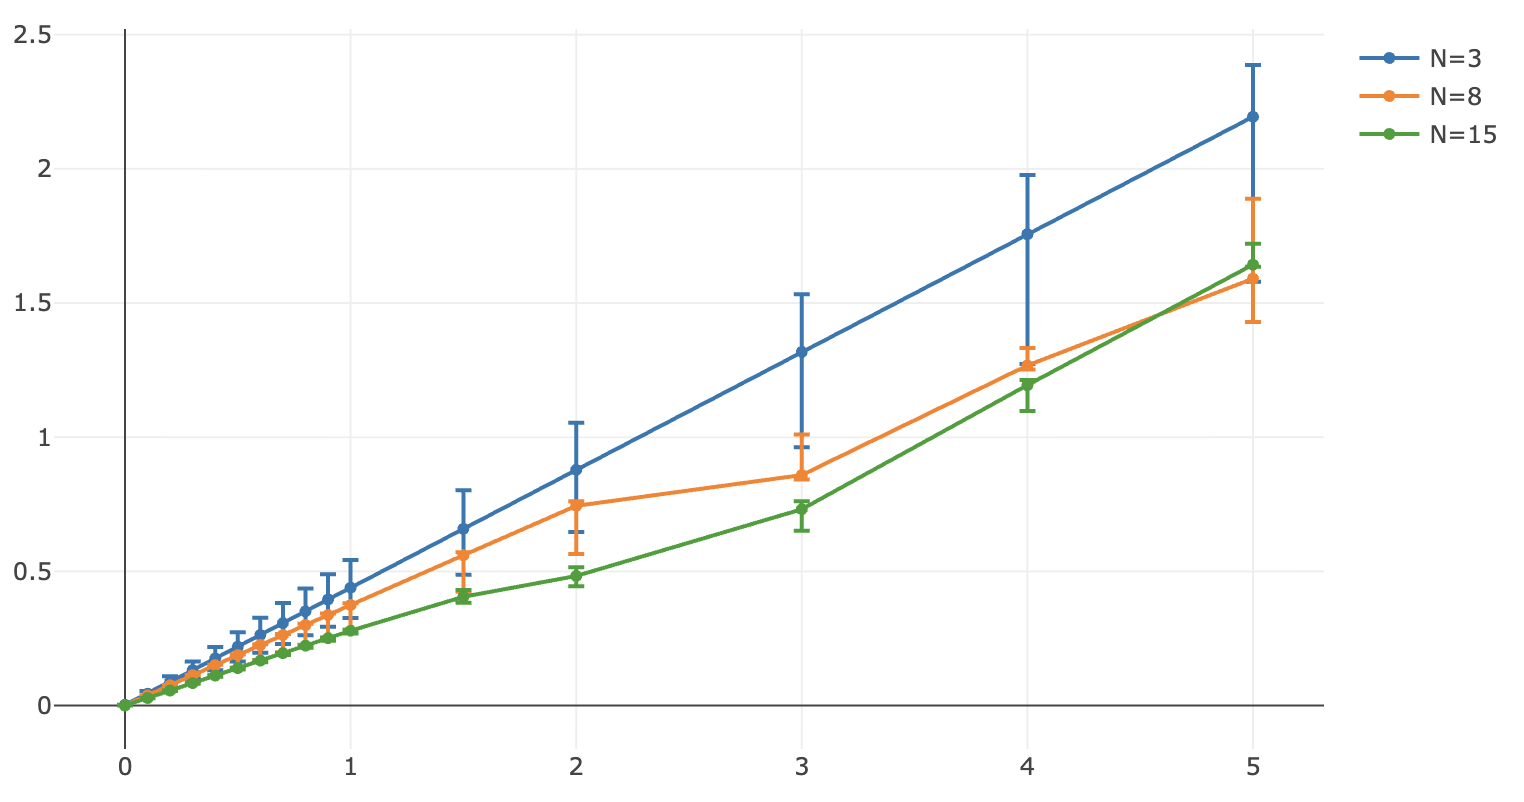
\includegraphics[width= 1\linewidth]{images'nshi/exp_b/b_various_nodes.png}
\caption{Graph depicting the Aligned Root Mean Square Error ($y$-$axis$) of the system with increasing noise values ($x$-$axis$). The blue line is the system with 3 active nodes, the yellow line is the system with 8 active nodes, while the green line is the system with 15 active nodes \label{fig:B_MAE}}
\end{figure}
As expected, the aligned RMSE increased monotonically with increasing noise. Across all noise levels, higher node density consistently yields lower localization error. This is particularly evident at higher noise values, where networks with more nodes exhibit significantly better robustness. At low noise levels, the system maintains high accuracy, with only minor degradation as $\sigma$ increases. This indicates that the spring-relaxation-based graph optimization is effective at absorbing small stochastic errors in the range measurements. However, beyond moderate noise levels, the error growth becomes more pronounced, reflecting the increasing difficulty of satisfying inconsistent distance constraints within the graph. The results demonstrate that the I.C.U.M localization approach degrades gracefully under increasing UWB noise. The approximately linear relationship between noise magnitude and final aligned error suggests predictable system behavior, which is desirable for real-world deployment. Notably, location information generally becomes more accurate the greater the number of active nodes in the system. Intuitively, this makes sense, as the more active nodes are present in the system, the more location information blinking nodes will receive, the greater the likelihood that the homogenised location values are correct. These results support the use of cooperative graph-based optimization for UWB localization in noisy environments and reinforce the system design choice of leveraging network redundancy to improve accuracy and stability, as outlined in earlier sections of the paper.

